\documentclass{ees}

\newgeometry{twoside=false,left=20mm,right=40mm,top=20mm,bottom=40mm}

\newlist{bulletlist}{itemize}{1}
\setlist[bulletlist]{
  partopsep=0pt,
  parsep=0pt,
  itemsep=0pt,
  label=\textbullet
}

\setcounter{tocdepth}{1}
\DeclareTOCStyleEntry[
  indent=0pt,
  beforeskip=\baselineskip,
  entrynumberformat=\@gobble,
  entryformat=\sbseries,
  numwidth=2em,
  linefill=\hfill,
  pagenumberbox=\pnumbox,
  pagenumberformat=\sbseries
]{tocline}{chapter}

\hyphenation{Musik-archiv}


\begin{document}

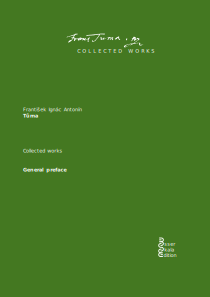
\includepdf{cover_general_preface.pdf}
\pagenumbering{arabic}
\setcounter{page}{1}

\tableofcontents

\chapter{General preface}

\textit{František Ignác Antonín Tůma: Collected works} (FIAT:CW) is an edition project that will make Tůma’s music available in modern editions. Simultaneously, it provides the source code used for typesetting the scores, thereby establishing a digital corpus of Tůma’s works that follows FAIR principles.

For more information, we refer the reader to our thematic catalogue of Tůma’s works, which is currently under development (\href{https://www.frantisek-tuma.at/}{https://www.frantisek-tuma.at/}). TumW numbers are cited from this catalogue.


\section{Editorial guidelines}

In general, FIAT:CW follows the \href{https://edition.esser-skala.at/about/editorial-guidelines/}{editorial guidelines} for the Edition Esser-Skala.


\section{Acknowledgements}

Assistance of the following people and institutions is gratefully acknowledged:
Thomas Dolezal (Dommusikarchiv Eisenstadt – A-Ed),
Ute-Eva Thiem (Benediktinerabtei Stift Göttweig, Musikarchiv – A-GÖ),
H. Ulrich Mauterer CanReg (Stift Herzogenburg, Musikarchiv – A-H),
P. Roman Nägele OCist (Stift Heiligenkreuz im Wienerwald, Musikarchiv – A-HE),
Martin Haltrich and Ulrike Wagner (Stift Klosterneuburg, Musikarchiv – A-KN),
P. Altman Pötsch OSB (Benediktinerstift Kremsmünster, Regenterei und Musikarchiv – A-KR),
Peter Deinhammer (Benediktinerstift Lambach, Musikarchiv – A-LA),
P. Michael Eppenschwandtner OSB (Benediktinerabtei Michaelbeuern, Musikarchiv – A-MB),
Christian Schüller (Röm.-Kath. Pfarramt Maria Taferl – A-MT),
P. Florian Ehebruster OSB (Benediktinerstift Seitenstetten, Musikarchiv – A-SEI),
Johannes Prominczel, Spiridoula Katsarou, and Günther Faimann (Archiv der Gesellschaft der Musikfreunde in Wien – A-Wgm),
Ikarus Kaiser (Stift Wilhering, Musikarchiv – A-WIL),
Michael Sipka (Erzbischöfliches Priesterseminar – A-Wps),
Maximilian Alexander Trofaier (Schottenstift Wien – A-Ws),
Stefan Engl and Ute Schmidthaler (Wienbibliothek im Rathaus, Musiksammlung – A-Wst),
Jan Jirák (Vlastivědné muzeum Dr. Hostaše v Klatovech, Klatovy – CZ-KLm),
Petr Slouka (Lobkowiczká knihovna a archiv, Nelahozeves – CZ-Nlob),
Ludmila Šmídová (Národní knihovna České republiky, Praha – CZ-Pu),
Christian Filips (Sing-Akademie zu Berlin, Notenarchiv – D-Bsa),
Christoph Hauser (Benediktinerabtei Ottobeuren, Bibliothek – D-OB),
Martin Lang (Bistum Passau, Archiv – D-Po),
Gábor Nemes (Székesegyházi Kottatár, Győr – H-Gk),
Orsolya Ódor, József Iván Kozma-Bognár, and Zsolt Bankó (Helikon Kastélymúzeum Könyvtára, Keszthely – H-KE),
Zoltán Damásdi (Pécsi Egyházmegye, Pécsi Püspöki Levéltár, Székesegyházi Kottatár – H-P),
Éva Samodai (Szent Benedek Rend Központi Főkönyvtára, Pannonhalma – H-PH),
Alessia Ravagnani (Museo internazionale e biblioteca della musica di Bologna – I-Bc),
Sebastian Lindblom (Musik- och teaterbiblioteket, Stockholm – S-Skma),
Kristína Hrivňáková (Archív mesta Bratislavy – SK-BRm),
Elisabeth Hilscher (Austrian Academy of Sciences),
David Gasche (Kunstuniversität Graz, Institut Oberschützen),
Vlastimil Tichý (Moravská zemská knihovna v Brně),
Jana Perutková (Masarykova Univerzita),
as well as the staff of
the Österreichische Nationalbibliothek, Musiksammlung, Wien (A-Wn),
the Moravská zemská knihovna v Brně (CZ-Bu),
the Státní okresní archiv, Ústí nad Orlicí (CZ-KRA/CZ-UO),
the Staatsbibliothek zu Berlin - Preußischer Kulturbesitz, Musikabteilung (D-B),
the Universität der Künste Berlin, Universitätsbibliothek, Berlin (D-Bhm),
the Sächsische Landesbibliothek - Staats- und Universitätsbibliothek, Dresden (D-Dl),
the Badische Landesbibliothek, Musiksammlung, Karlsruhe (D-KA),
the Universitetsbiblioteket Lund (S-L),
and the Boston Public Library, Music Department (US-Bp).


\clearpage
\markdownInput{../CHANGELOG.md}

\end{document}
